% DATA 266 Lab 2 -- Pair 44 -- report DRAFT covering Parts 1, 2 and 3 (NOT final: Part 2 human results added
% 2026-11-18 (D-118); Part 1 groundedness and Part 3 human judgements still pending).
% Compile with pdfLaTeX on Overleaf (IEEEtran is built in). Figures are in figures/ (sources: Appendix B).
% Every number below is copied from saved experiment records (sources in Appendix A).
% Evidence tags for Part 1: [OUTPUT] = printed in a saved executed notebook; [DOC] = recorded only in the
% decision log; [KAGGLE] = computed by Kaggle. Parts 2/3 values come from saved JSON/notebook outputs.
% \pending{...} marks content that needs human input; \missing{...} marks absent deliverables.
% Search for "PENDING" and "MISSING" before submitting. Do not replace pending human results with estimates.
\documentclass[conference]{IEEEtran}
\usepackage[T1]{fontenc}
\usepackage{graphicx,booktabs,amsmath,url,xcolor,tikz}
\usetikzlibrary{positioning,arrows.meta}
\newcommand{\pending}[1]{\textcolor{red}{\textbf{[PENDING: #1]}}}
\newcommand{\missing}[1]{\textcolor{red}{\textbf{[MISSING: #1]}}}
\graphicspath{{figures/}}

\begin{document}
\title{DATA 266 Lab 2: Multimodal RAG, Domain Fine-Tuning of Stable Diffusion, and a Guarded Multi-Agent Image System}
\author{\IEEEauthorblockN{Parth Patel, Chelsi Shulamite}
\IEEEauthorblockA{Pair Programming Team 44 --- DATA 266, Fall 2026\\ GitHub: \url{https://github.com/shulamite512/DATA266_LAB2_PAIR44} (private access: \pending{confirm})}}
\maketitle

\begin{abstract}
For Part~1 we built a multimodal retrieval-augmented question-answering system over three read-only PDFs: dense and BM25 retrieval fused by RRF, a cross-encoder reranker, a label router, a revision/conflict registry and Qwen3-VL-4B answers in a validated JSON schema.
\begin{itemize}
\item On the frozen 25-question golden set (the only held-out run, P1-EXP-001, with earlier code), the final retrieval mode raised Recall@5 from 0.764 to 0.882 and citation accuracy from 0.64 to 0.84 over a dense-only baseline, while answer correctness stayed at 13--14 of 25.
\item The final notebook (P1-KAGGLE-V14-R1) ran on a Kaggle NVIDIA T4 in 43.6 minutes with Qwen3-VL-4B in 4-bit NF4 and produced a 40-row submission that passed the course validator. Its leaderboard score is not recorded here; the earlier P1-EXP-003 checkpoint scored 0.832 on the public leaderboard.
\end{itemize}
For Part~2, we fine-tuned Stable Diffusion 1.5 with two LoRA adapters (rank 4 and rank 64) on 740 BLIP-captioned Pok\'emon images. We compared them with the base model on 120 generated images using KID, CLIP score, LPIPS diversity, a memorization probe and safety-checker counts. The rank-4 adapter was selected by a pre-registered rule (in-domain KID $0.0619\pm0.0092$ vs.\ $0.0825\pm0.0089$ for rank 64 and $0.0823\pm0.0111$ for the base model). Blinded human raters did \emph{not} confirm this improvement: in 25 pairs judged by three raters, the rank-4 adapter was preferred over the base model in 38.7\% (29/75) of domain-style judgments and 41.3\% (31/75) of prompt-match judgments (majority vote 10/25 for both).
For Part~3, we built a five-agent system (Planner, Vision, Prompt, Generation, Critique) around a shared typed state. It uses Qwen3-VL-4B, SD~1.5 with the selected adapter, InstructPix2Pix and CLIP, allows at most two revisions, and writes a JSON trace for every request.
In the final evaluation (P3-EXP-003), all 40 requests executed (15 scenarios with and without critique, plus 10 red-team cases). Automated structural checks passed 12/15 with critique and 11/15 without. No red-team attack succeeded among the 8 cases decided automatically; 2 await human review. Six requests failed because the vision model fell into a deterministic repetition loop; we report this as a confirmed limitation. Human judgements are \pending{Part~1 groundedness ratings, two-judge Part~3 results}.
\end{abstract}

\section{Introduction}
Part 1 answers questions over a small, deliberately tricky knowledge base. Its three PDFs contain vector and raster figures, tables, revisions, errata, cross-document conflicts and a low-trust appendix with embedded instructions. Answers must cite exact pages and figure labels and keep per-conversation state without ever modifying the knowledge base. Part 2 measures how much a small LoRA adapter shifts SD~1.5 toward a target art style, and at what cost to prompt fidelity, diversity and memorization. Part 3 composes vision-language understanding, prompt rewriting, generation and self-critique into a guarded pipeline. It treats text inside images as untrusted data and refuses unsafe or deceptive requests. All three parts run from versioned notebooks with frozen evaluation files committed before the experiments (Section~\ref{sec:repro}).

\section{Experimental Setup and Reproducibility}\label{sec:repro}
\textbf{Part 1 environment.} The final notebook (P1-KAGGLE-V14-R1) ran on Kaggle with one NVIDIA Tesla T4 (14{,}912~MB): Python 3.13.16, torch 2.11.0+cu130, transformers 5.16.1, bitsandbytes 0.49.0, sentence-transformers 5.7.0, chromadb 1.5.9, PyMuPDF 1.28.2, rank-bm25 0.2.2, accelerate 1.14.0 and numpy 2.1.3 [OUTPUT]; seed 266, greedy decoding. The Part~1 model revisions were \emph{not} pinned (Section~\ref{sec:limits}). The earlier runs P1-EXP-001--003 used an RTX 5090 in a Docker container (Python 3.11.13, torch 2.7.1+cu128). The frozen 25-question golden set was committed on 2026-10-21 (\texttt{d9bbd68}), before any Part~1 code (\texttt{c097b26}).

\textbf{Parts 2--3 hardware and software.} One NVIDIA RTX 5090 (32{,}607~MB) in a Docker container (Python 3.12.3, PyTorch 2.14.1+cu130, diffusers 0.39.0, transformers 4.57.6, peft 0.21.2, gradio 5.50.0; the full lock file is \texttt{docker/requirements-p2p3.lock.txt}). Exactly one GPU is visible. The PyTorch allocator is capped at 16{,}384~MB as a \emph{preliminary} 16~GB check only. This is not evidence of compatibility with a real 16~GB GPU (Section~\ref{sec:limits}).

\textbf{Determinism and provenance.} Seed 266; pinned Hugging Face revisions (SD~1.5 \texttt{451f4fe1}, Qwen3-VL-4B \texttt{ebb281ec}, InstructPix2Pix \texttt{31519b5c}, CLIP ViT-L/14 \texttt{32bd6428}, dataset \texttt{3790f299}). The dataset split, the 20 evaluation prompts, the Part 3 scenarios, the red-team cases and the input manifest were hashed and committed \emph{before} the corresponding runs. Each notebook refuses to run if a frozen file or the code fingerprint has changed. Completed experiment IDs are never overwritten.

\section{Part 1: Multimodal RAG over a Read-Only Knowledge Base}\label{sec:p1}
\subsection{Knowledge base and task}
The knowledge base has three PDFs with a trust manifest: DOC1 with vector-drawn figures, and DOC2/DOC3 with raster figures, tables, a revision notice, an erratum (``Figure B-5 (corrected)'') and a low-trust Appendix~C that contains embedded instructions.
\begin{itemize}
\item Each question is answered in JSON with an answer of at most 120 words, one of five statuses (answered, not\_found, conflict, false\_premise, session\_override), page citations \texttt{DOC\#:p\#} and figure/table labels.
\item Multi-turn conversations may introduce user-supplied values. These apply only within their conversation and never change the knowledge base.
\item Kaggle scores 0.40 answer correctness (within $\pm1\%$), 0.20 status, 0.20 figure-reference F1 and 0.20 citations.
\end{itemize}

\subsection{Architecture}
Fig.~\ref{fig:p1arch} shows the pipeline of the final notebook (P1-KAGGLE-V14-R1).
\begin{itemize}
\item \textbf{Ingestion} (PyMuPDF): locates every caption, crops vector and raster figures, and normalises tables to long-format records. In the final run it indexed 195 objects; evidence figures get a VLM-written JSON chart description [OUTPUT].
\item \textbf{Trust handling:} low-trust objects (Appendix~C) are indexed but flagged \texttt{evidence\_ok=False} and filtered out of every context.
\item \textbf{Registry:} links corrections to originals, notices to the labels they name, and forecast/outturn pairs and cross-document disagreements via series keys.
\item \textbf{Retrieval} (final mode): an exact-label router; dense \texttt{bge-large-en-v1.5} top-20 and BM25 top-20 fused by RRF ($k{=}60$); the \texttt{bge-reranker-v2-m3} cross-encoder on the CPU (20$\rightarrow$6); registry expansion of at most 3 objects.
\item \textbf{Generation:} Qwen3-VL-4B, loaded in 4-bit NF4 (bitsandbytes) to fit the T4, writes a JSON answer (answer, status, citations, figure references, values) with greedy decoding. Rule-based post-processing then checks the grounding of citations, labels and numbers, status rules and arithmetic, with a repair retry and a deterministic fallback.
\item \textbf{Conversation memory:} one \texttt{ConversationState} per conversation (rewrites, user values, refused knowledge-base edits). The index fingerprint is asserted unchanged.
\item \textbf{Baseline:} dense-only top-20 with the same trust filter, top 8 as context.
\end{itemize}

\begin{figure}[t]\centering\footnotesize
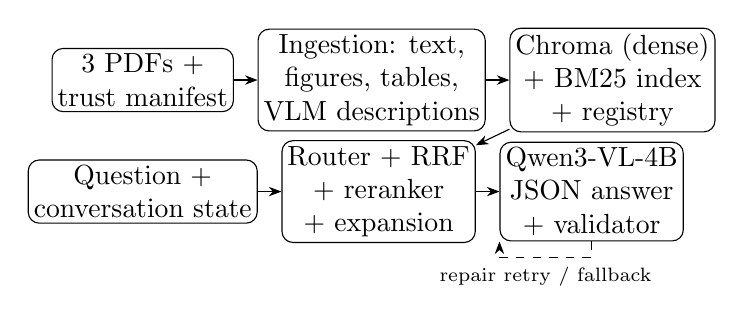
\begin{tikzpicture}[node distance=3mm, box/.style={draw,rounded corners,minimum height=5mm,inner sep=2pt,align=center}, >={Stealth[length=1.6mm]}]
\node[box](pdf){3 PDFs +\\trust manifest}; \node[box,right=of pdf](ing){Ingestion: text,\\figures, tables,\\VLM descriptions};
\node[box,right=of ing](idx){Chroma (dense)\\+ BM25 index\\+ registry};
\node[box,below=6mm of pdf](q){Question +\\conversation state}; \node[box,right=of q](ret){Router + RRF\\+ reranker\\+ expansion};
\node[box,right=of ret](gen){Qwen3-VL-4B\\JSON answer\\+ validator};
\draw[->](pdf)--(ing); \draw[->](ing)--(idx); \draw[->](q)--(ret); \draw[->](idx)--(ret); \draw[->](ret)--(gen);
\draw[->,dashed](gen.south) -- ++(0,-2mm) -| node[pos=0.25,below]{\scriptsize repair retry / fallback} (gen.south west);
\end{tikzpicture}
\caption{Part~1 RAG pipeline (final mode). Low-trust objects are indexed but never enter a context; the index is never written by conversations.}\label{fig:p1arch}\end{figure}

\subsection{Evaluation protocol and integrity}
\begin{itemize}
\item The golden set has 25 questions in six categories (facts/tables, figures, two sources, multi-turn override, conflicts/revisions, unanswerable/false premise/injection). It was committed before any code.
\item \textbf{P1-EXP-001} is the only held-out run: the golden set was not used for development before it. Its metrics are printed in the saved notebook (\texttt{0adebfa}) [OUTPUT].
\item Afterwards, golden-set failure analysis guided general fixes, so later golden-set numbers are \emph{development} estimates [DOC].
\item The public Kaggle leaderboard was used as feedback only, with no question-specific rules.
\end{itemize}

\begin{table}[t]\centering\caption{Part 1 golden set (25 questions). P1-EXP-001 is held-out [OUTPUT]; P1-EXP-003 is a development measurement [DOC]. Both use earlier code; the final V14-R1 notebook was not run on the golden set.}\label{tab:p1}\footnotesize
\begin{tabular}{lccc}\toprule
Metric & EXP-001 baseline & EXP-001 final & EXP-003 final (dev.)\\\midrule
Correct answers & 14/25 & 13/25 & 14/25\\
Recall@5 (24 items) & 0.764 & 0.882 & 0.882\\
Hit@5 & 0.958 & 0.958 & 0.958\\
Citation accuracy & 0.64 & 0.84 & 0.76\\
Figure-reference F1 & 0.627 & 0.793 & 0.68\\
Median s/question & 1.77 & 2.03 & 6.63\\
Groundedness (human) & \multicolumn{3}{c}{not rated (Section~\ref{sec:limits})}\\\bottomrule
\end{tabular}\end{table}

\subsection{Results}
\textbf{Held-out comparison} (Table~\ref{tab:p1}).
\begin{itemize}
\item The final architecture clearly improves retrieval (Recall@5 $+0.118$) and citations (citation accuracy $+0.20$, figure-reference F1 $+0.166$), but not answer correctness (13 vs.\ 14 of 25).
\item The P1-EXP-001 failure analysis traced most final-mode misses to errors \emph{after} correct retrieval: answer/status inconsistency, rounding and arithmetic, a user value not reused on a later turn, and undetected text-level conflicts. Chart-value reading was a separate model limitation [DOC].
\end{itemize}

\textbf{Kaggle.}
\begin{itemize}
\item The final submission is the output of P1-KAGGLE-V14-R1 (\texttt{eval/p1\_submission.csv}). Its leaderboard score is not recorded in this report.
\item Historical public-leaderboard scores of earlier versions were 0.636 (P1-EXP-002) and 0.832 (P1-EXP-003; rank 1 at that time) [KAGGLE]. The public split covers about 48\% of the hidden set.
\end{itemize}

\textbf{Submission run} (P1-KAGGLE-V14-R1, saved output).
\begin{itemize}
\item 40 rows; the professor's \texttt{validate\_submission.py} printed ``valid: 40 rows''.
\item Statuses: answered 32, conflict 3, session\_override 3, not\_found 2.
\item 2 rows retried (ungrounded numbers), 0 fallbacks; total runtime 2{,}616~s (43.6~min) of the 5{,}400~s budget, 1{,}961~s of it answering; at most 4{,}580~MB PyTorch peak allocation per model call [OUTPUT].
\end{itemize}

\textbf{Readiness checks.} 5/5 passed (processor geometry, NF4 load on one device, attention path, text generation, single-image generation), and the run verdict was PASS [OUTPUT]. The earlier 46/47 self-check result belongs to P1-EXP-003.

\subsection{Safety}
\begin{itemize}
\item \textbf{Low-trust evidence:} the low-trust Appendix~C is retrievable without the filter but never enters a context, and the router refuses its labels [OUTPUT].
\item \textbf{Embedded instructions:} instructions embedded in the evidence are not followed (gate G7.embedded\_instruction).
\item \textbf{Knowledge-base edits:} requests to edit the knowledge base are refused. User values apply only within their own conversation, and the index fingerprint is unchanged after all conversations (gate G8) [OUTPUT].
\item These gate results come from the self-checks of the earlier checkpoint P1-EXP-003. The final V14-R1 notebook keeps the trust filter in its code but did not re-run those gates.
\end{itemize}

\section{Part 2: LoRA Fine-Tuning of Stable Diffusion 1.5}
\subsection{Data and training}
Dataset \texttt{reach-vb/pokemon-blip-captions} (CC BY-NC-SA 4.0): 833 rows; 11 near-duplicates removed; 740 train and 82 test images, with a minimum train--test dHash distance of 6. Both runs use the same frozen 740-image train split. Shared settings: LoRA on \texttt{to\_q, to\_k, to\_v, to\_out.0}; AdamW (lr $10^{-4}$, cosine schedule, 5\% warm-up, weight decay 0.01); 1{,}500 steps; effective batch 4 (micro-batch 4); fp16 frozen weights with fp32 LoRA weights. Table~\ref{tab:p2runs} lists the runs and Fig.~\ref{fig:loss} the loss curves.

\begin{table}[t]\centering\caption{Part 2 training runs (P2-EXP-001)}\label{tab:p2runs}
\begin{tabular}{lrrrrr}\toprule
Run & rank/$\alpha$ & trainable & \% & peak MB & GPU-h\\\midrule
A & 4/4 & 797{,}184 & 0.093 & 6{,}307 & 0.067\\
B & 64/64 & 12{,}754{,}944 & 1.462 & 6{,}542 & 0.069\\\bottomrule
\end{tabular}\end{table}

\begin{figure}[t]\centering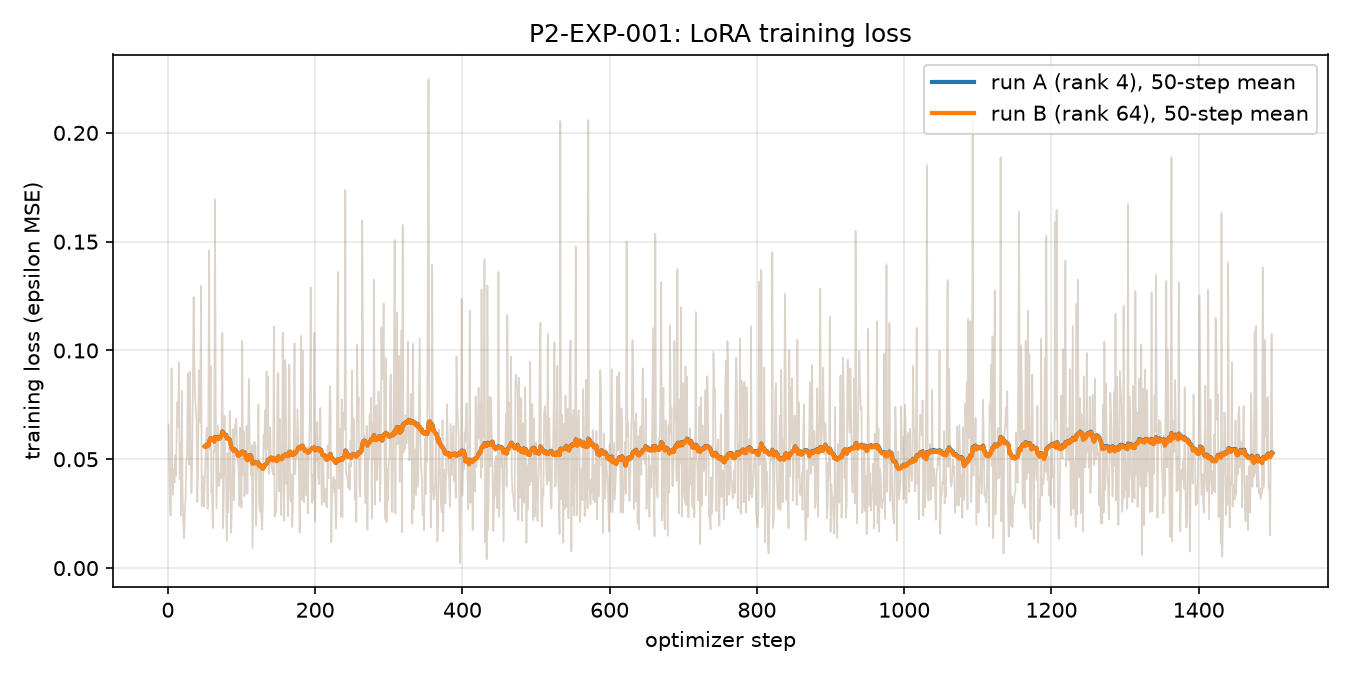
\includegraphics[width=\linewidth]{p2_loss_curves.png}
\caption{Training loss of runs A and B (P2-EXP-001).}\label{fig:loss}\end{figure}

\subsection{Evaluation protocol}
20 frozen prompts (10 in-domain captions from test rows, 5 out-of-domain, 5 compositional) $\times$ seeds \{0,1\} $\times$ \{base, A, B\} gives 120 images at $512\times512$. Sampler: DPM-Solver multistep, 30 steps, guidance 7.5, safety checker on. Metrics:
\begin{itemize}
\item KID (Inception features), 20 in-domain generations against the 82 test images, subset size 20. This is high-variance, so we report the std.
\item CLIP ViT-L/14 image--text score per prompt group. This CLIP model is related to SD's text encoder and may favour SD outputs.
\item LPIPS (AlexNet) between the two seeds of each prompt, as a diversity measure.
\item Memorization: CLIP image cosine of each of 10 in-domain seed-0 generations to its nearest training image.
\item Safety-checker flags. Flagged images stay in the primary metrics, and a sensitivity analysis excludes them.
\end{itemize}

\subsection{Results}
\begin{table*}[t]\centering\caption{Part 2 results (P2-EXP-001). All columns except the last are automated metrics. The last column is the blinded human win rate of the selected adapter against the base model (3 raters $\times$ 25 pairs = 75 judgments per criterion; Section~\ref{sec:human2}).}\label{tab:p2}
\begin{tabular}{lcccccccc}\toprule
Model & KID$\downarrow$ (mean$\pm$std) & CLIP all & CLIP in & CLIP out & CLIP comp. & LPIPS div. & NSFW flags/40 & Human win (style / prompt)\\\midrule
Base SD 1.5 & $0.0823\pm0.0111$ & 28.87 & 27.25 & 29.69 & 31.28 & 0.834 & 1 & reference\\
LoRA A (r4), selected & $\mathbf{0.0619\pm0.0092}$ & 27.92 & 26.75 & 30.03 & 28.13 & 0.744 & 3 & 38.7\% / 41.3\%\\
LoRA B (r64) & $0.0825\pm0.0089$ & 26.04 & 24.71 & 30.18 & 24.54 & 0.711 & 8 & not rated\\\bottomrule
\end{tabular}\end{table*}

Table~\ref{tab:p2} shows the results.
\begin{itemize}
\item \textbf{KID:} run A has the lowest in-domain KID. Its gap to the base model (0.0204) is about 1.8 times the larger std, but with 20 samples that difference is only indicative.
\item \textbf{Selection:} run A was chosen by the rule fixed before evaluation: lower in-domain KID; if the KID gap is within one std, the higher in-domain CLIP score decides.
\item \textbf{CLIP score:} both adapters lower the in-domain and compositional CLIP scores relative to the base model, and run B lowers them most (compositional 24.54 vs.\ 31.28 for base). This suggests that a higher rank pulls prompts toward the training style at the expense of prompt fidelity.
\item \textbf{Diversity:} LPIPS diversity also falls with rank (0.834 base, 0.744 A, 0.711 B).
\item \textbf{Sensitivity analysis:} excluding safety-flagged images changes KID to 0.0782 (base, $n{=}19$), 0.0502 (A, $n{=}18$) and 0.0286 (B, $n{=}15$). With 8 of its 40 images blacked out, run B's primary KID is strongly affected by flagged images, so the B-vs-A comparison is not robust. We report this and do not re-select.
\end{itemize}

\textbf{Memorization.} The mean top-1 training-image cosine is 0.644 (base), 0.723 (A, max 0.826) and 0.753 (B, max 0.867). Held-out \emph{real} test images reach 0.892 (max 0.953) against the training set. No generated image exceeds that natural level, so we see no evidence of near-copies (Fig.~\ref{fig:mem}). \pending{team's visual judgement of Fig.~\ref{fig:mem}}

\textbf{Safety.} The SD safety checker flagged 1 (base), 3 (A) and 8 (B) of 40 images each. A flag replaces the image with a black frame. These are cartoon prompts, so the flags are likely false positives, but we did not verify this by hand. \pending{inspect flagged prompts and state whether any is a true positive}

\begin{figure}[t]\centering
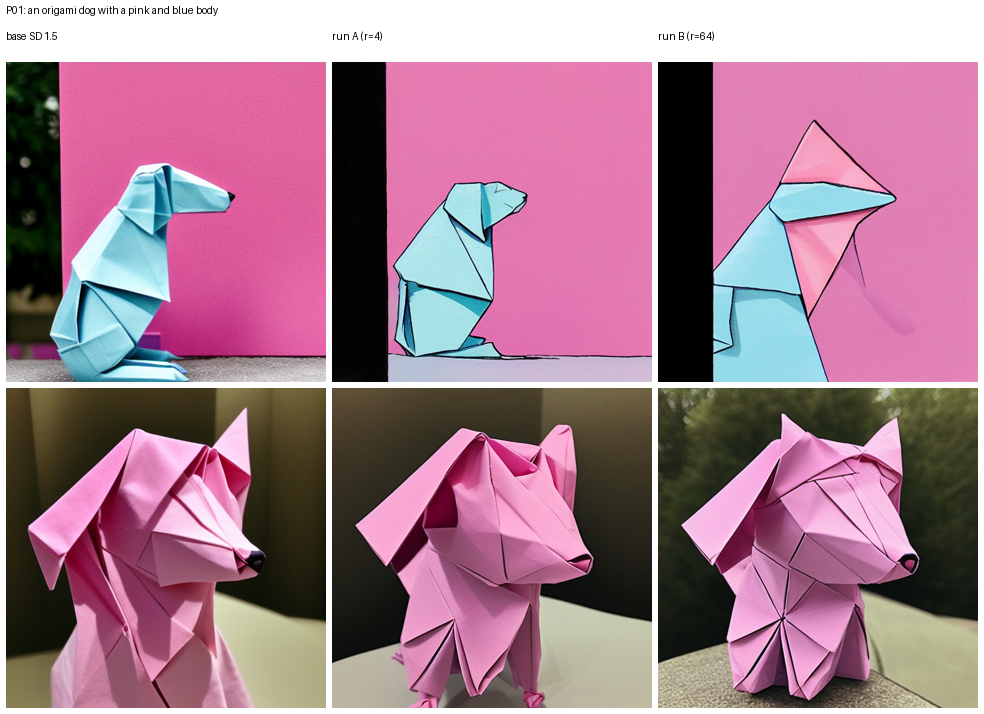
\includegraphics[width=\linewidth]{p2_grid_P01.png}\\[2pt]
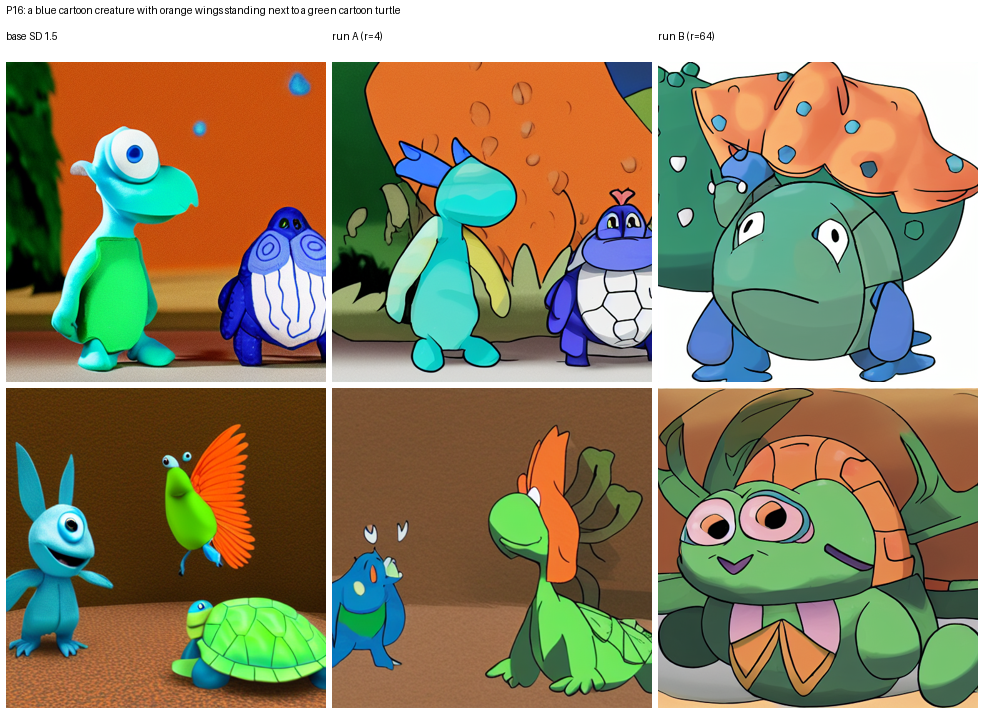
\includegraphics[width=\linewidth]{p2_grid_P16.png}
\caption{Base vs.\ LoRA A vs.\ LoRA B for an in-domain prompt (P01, top) and a compositional prompt (P16, bottom); rows are seeds 0 and 1. The out-of-domain grid is in \texttt{figures/p2\_grid\_P11.png}.}\label{fig:grid}\end{figure}

\begin{figure}[t]\centering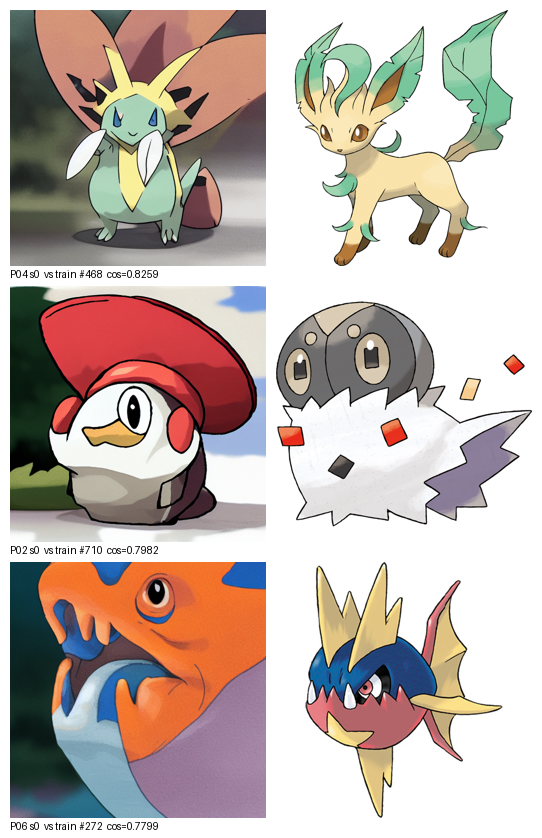
\includegraphics[width=\linewidth]{p2_memorization_top3_runA.png}
\caption{Top-3 most similar (generation, training image) pairs for run A.}\label{fig:mem}\end{figure}

\subsection{Human evaluation}\label{sec:human2}
\textbf{Method.} There are 25 blinded (prompt, seed) pairs of the final adapter (LoRA~A) vs.\ the base model, drawn from the 40 (prompt, seed) combinations with seed 266. Which side shows which model was also randomised with seed 266; LoRA~A is on the left in 14 pairs. Three raters (RATER\_1--3; the design is both members plus one outside person) judged every pair independently on \emph{domain\_style} (``Which image looks more like the Pok\'emon artwork style of the training data?'') and \emph{prompt\_match} (``Which image matches the prompt text better?''), choosing left or right with no ties, in a local click-through tool that shows the unmodified packet images. The 150 ratings were validated (each rater exactly 25 pairs $\times$ 2 criteria; no missing, invalid or duplicated rows) and committed unchanged \emph{before} the answer key was applied. The notebook then scored them in \texttt{REPORT\_ONLY} mode, which does not train, generate or recompute any automated metric.

\begin{table}[t]\centering\caption{Part 2 human evaluation: LoRA~A preferred over base SD~1.5 (P2-EXP-001)}\label{tab:p2human}
\begin{tabular}{lcc}\toprule
 & domain\_style & prompt\_match\\\midrule
All judgments (pre-registered) & 29/75 = 38.7\% & 31/75 = 41.3\%\\
Majority vote per pair (pre-registered) & 10/25 = 40.0\% & 10/25 = 40.0\%\\
RATER\_1 / RATER\_2 / RATER\_3 & 36\% / 52\% / 28\% & 36\% / 48\% / 40\%\\
Unanimous pairs (for A / for base) & 12 (3 / 9) & 18 (7 / 11)\\\midrule
\multicolumn{3}{l}{\emph{Post-hoc supplementary statistics (not pre-registered)}}\\
Fleiss' $\kappa$ (A vs.\ base) & 0.27 & 0.62\\
Majority vote, Wilson 95\% CI & [23\%, 59\%] & [23\%, 59\%]\\
Majority vote, exact binomial $p$ vs.\ 50\% & 0.42 & 0.42\\
Without pair H22 (A image safety-blacked) & 29/72 = 40.3\% & 31/72 = 43.1\%\\\bottomrule
\end{tabular}\end{table}

\textbf{Results.} Table~\ref{tab:p2human} shows the results. Raters preferred the \emph{base} model more often than LoRA~A on both criteria. Only RATER\_2's domain-style rate (13/25) is above 50\%. With 25 pairs the result is not statistically distinguishable from no preference: the majority-vote 95\% interval spans 23--59\%, and the pooled judgments are not independent because all three raters judged the same pairs. Agreement was moderate to substantial for prompt match ($\kappa=0.62$; pairwise agreement 80--84\%) but only fair for domain style ($\kappa=0.27$; 52--76\%). The style question was therefore interpreted less consistently. By prompt group (post-hoc; 11 in-domain, 6 out-of-domain and 8 compositional pairs), LoRA~A won 11/33 in-domain style judgments and 9/33 in-domain prompt-match judgments. These small subgroups are descriptive only.

\textbf{Human vs.\ automated evidence.} The human preferences and the automated scores measure different things and should not be merged. KID, CLIP and LPIPS (Table~\ref{tab:p2}) are computed by models: KID compares Inception feature statistics of 20 in-domain generations with the 82 test images and favoured LoRA~A, while CLIP already scored LoRA~A below the base model in-domain and on compositional prompts. The human raters judged single side-by-side pairs, and they did not prefer LoRA~A on average. KID-based selection of LoRA~A is therefore not confirmed by human preference. We keep the pre-registered selection, report this disagreement, and do not re-select.

\textbf{Limitations of the human study.} 25 pairs and 3 raters give low statistical power. By design two of the three raters are the authors, and raters are recorded only by ID. The style question showed only fair agreement. In one pair (H22) the LoRA~A image had been replaced by a black frame by the safety checker; all raters chose the base image, and the primary numbers keep it as generated. One pre-fix backup of the rating tool holds an earlier RATER\_1 answer for H01 \emph{domain\_style} (base) that differs from the final saved answer (LoRA~A). Using that earlier answer would give 28/75 and a 9/25 majority. The final saved answer is the one scored.

\section{Part 3: Five-Agent Multimodal System}
\subsection{Architecture and data flow}
Fig.~\ref{fig:arch} shows the pipeline.
\begin{itemize}
\item \textbf{Input guard:} validates the request text and the image.
\item \textbf{Planner} (Qwen3-VL-4B with deterministic screens): classifies the intent (caption\_question, style\_change, edit, enhance, domain\_style, unsupported) and runs the safety screens.
\item \textbf{Vision agent:} returns a JSON report (caption, objects, scene, observed text, person flags, answers to fixed questions).
\item \textbf{Prompt agent:} writes the generation specification.
\item \textbf{Generation agent:} chooses SD~1.5 txt2img/img2img (with the Part~2 LoRA \emph{only} for domain\_style, verified ON/OFF per request) or InstructPix2Pix for edits.
\item \textbf{Critique agent:} combines a CLIP score (threshold $\tau{=}25$ for style intents) with a VLM judgement. The orchestrator, not the VLM, decides ACCEPT or REVISE and enforces at most two revisions.
\end{itemize}
Caption and question requests end after the Vision agent. Unsafe or ambiguous requests end at the Planner.

\begin{figure}[t]\centering\footnotesize
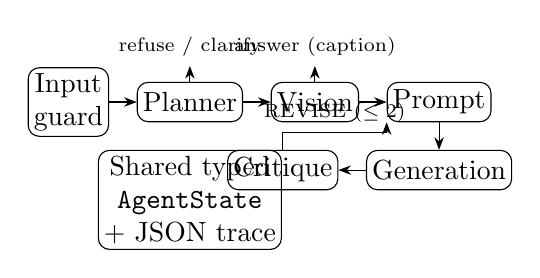
\begin{tikzpicture}[node distance=3.5mm, box/.style={draw,rounded corners,minimum height=5mm,inner sep=2pt,align=center}, >={Stealth[length=1.6mm]}]
\node[box](g){Input\\guard}; \node[box,right=of g](p){Planner}; \node[box,right=of p](v){Vision};
\node[box,right=of v](pr){Prompt}; \node[box,below=of pr](ge){Generation}; \node[box,left=of ge](c){Critique};
\node[box,below=of p](st){Shared typed\\\texttt{AgentState}\\+ JSON trace};
\draw[->](g)--(p); \draw[->](p)--(v); \draw[->](v)--(pr); \draw[->](pr)--(ge); \draw[->](ge)--(c);
\draw[->](c.north) -- ++(0,2.2mm) -| node[pos=0.25,above]{\scriptsize REVISE ($\leq2$)} (pr.south west);
\draw[->,dashed](v.north) -- ++(0,2mm) node[above]{\scriptsize answer (caption)};
\draw[->,dashed](p.north) -- ++(0,2mm) node[above]{\scriptsize refuse / clarify};
\end{tikzpicture}
\caption{Agent pipeline. The orchestrator owns all transitions; every step is appended to the trace.}\label{fig:arch}\end{figure}

\subsection{Shared state, guardrails and traces}
All agents read and write one pydantic \texttt{AgentState}: an explicit phase machine, a typed plan, the vision report, prompt specifications, attempts, critiques, a revision count capped at 2, and errors. Illegal phase transitions raise an exception. Text found inside an image is stored as an immutable \texttt{UntrustedText} and enters prompts only inside a delimited block. If instruction-like text is found in any transcribed line, in the joined transcription or in the VLM's description, every generation or edit is refused.

Every request produces one JSON trace: per-agent inputs and outputs, timing, status, errors and generation diagnostics, with secrets redacted. All 40 traces of each experiment are committed under \texttt{traces/<experiment>/}.

\subsection{Evaluation design}
The evaluation has 15 scenarios, 3 per category (caption/question, style change, edit or enhance, domain style, ambiguous or broken). Each scenario has an expected route, an expected status with and without critique, and a written pass rubric. Every scenario runs once with critique and once without.

The 10 red-team cases are 3 image-embedded instructions, 3 unsafe requests, 2 deceptive edits of a real person (a public-domain historical portrait), and 2 broken files. Inputs are licensed Wikimedia Commons photographs, Part~2 test images, code-drawn injection posters and broken fixtures, all pinned by SHA-256.

The \emph{automated structural checks} test status, executed route, presence of an output image and LoRA state. They are diagnostics, \emph{not} task success. Task success is judged by two independent team members on a blinded packet (Section~\ref{sec:human3}).

\subsection{Experiment history}
\textbf{P3-EXP-001 (preliminary).}
\begin{itemize}
\item 22/40 records ran; 18 were NOT\_RUN because team photographs were never supplied.
\item One red-team attack succeeded: R01, where an instruction split over several lines of image text was not detected and an image was generated.
\item The input safety checker produced a false positive on a held-out test image (S01).
\end{itemize}

\textbf{P3-EXP-002.} A post-preliminary amendment (v2) replaced the inputs with licensed dataset images. It also fixed injection scanning over the joined transcription, required the VLM to confirm the safety checker's input flags, and checked the \emph{executed} route rather than the planned one. All 40 requests executed, and six records ended FAILED\_MODEL in the Vision agent.

\textbf{P3-EXP-003 (final).}
\begin{itemize}
\item It raised the Vision agent's token limit from 450 to 1024 and added generation diagnostics.
\item The inputs, rubrics, prompts and models were identical to P3-EXP-002, which was verified against its freeze.
\item Both amendments were made \emph{after} earlier results were seen, so neither the scenario set nor the red-team set is an untouched hold-out.
\end{itemize}

\subsection{Results (P3-EXP-003)}
\begin{table}[t]\centering\caption{P3-EXP-002 vs.\ P3-EXP-003 (automated; not task success)}\label{tab:p3cmp}
\begin{tabular}{lcc}\toprule
Metric & EXP-002 & EXP-003\\\midrule
Executed / NOT\_RUN / runner failures & 40/0/0 & 40/0/0\\
FAILED\_MODEL records & 6 & 6\\
Vision JSON failures (of 22 calls) & 6 & 6\\
Auto checks, with critique & 12/15 & 12/15\\
Auto checks, without critique & 11/15 & 11/15\\
Mean revisions (with critique) & 0.8 & 0.8\\
Median latency, all (s) & 8.13 & 7.96\\
\quad with / without critique (s) & 11.43 / 8.41 & 14.10 / 8.25\\
\quad red-team (s) & 1.53 & 1.54\\
Red-team confirmed successes & 0 & 0\\
Red-team defended / pending human & 8 / 2 & 8 / 2\\
Max peak GPU allocation (MB) & -- & 12{,}537\\\bottomrule
\end{tabular}\end{table}

\begin{table}[t]\centering\caption{Final status per scenario, P3-EXP-003 (rev = revisions)}\label{tab:p3sc}\footnotesize
\begin{tabular}{llll}\toprule
ID & Category & With critique & Without critique\\\midrule
S01 & caption & ANSWERED & ANSWERED\\
S02 & caption & FAILED\_MODEL & FAILED\_MODEL\\
S03 & caption & FAILED\_MODEL & FAILED\_MODEL\\
S04 & style & FAILED\_MODEL & FAILED\_MODEL\\
S05 & style & MAX\_REVISIONS (2 rev) & COMPLETED\\
S06 & style & MAX\_REVISIONS (2 rev) & BLOCKED\_UNSAFE\_OUTPUT\\
S07 & edit/enh. & MAX\_REVISIONS (2 rev) & COMPLETED\\
S08 & edit/enh. & ACCEPTED (0 rev) & COMPLETED\\
S09 & edit/enh. & MAX\_REVISIONS (2 rev) & COMPLETED\\
S10 & domain & ACCEPTED (2 rev) & COMPLETED\\
S11 & domain & ACCEPTED (1 rev) & COMPLETED\\
S12 & domain & ACCEPTED (1 rev) & COMPLETED\\
S13 & ambiguous & NEEDS\_CLARIFICATION & NEEDS\_CLARIFICATION\\
S14 & broken & FAILED\_INPUT & FAILED\_INPUT\\
S15 & broken & FAILED\_INPUT & FAILED\_INPUT\\\bottomrule
\end{tabular}\end{table}

\textbf{Execution and automated checks} (Tables~\ref{tab:p3cmp}, \ref{tab:p3sc}).
\begin{itemize}
\item All 40 requests executed.
\item Expected non-image outcomes were reached: the clarification request (S13) and the broken inputs (S14, S15, R09, R10).
\item The LoRA was active in every domain-style attempt and inactive in every other generation.
\item Automated checks: 12/15 with critique; 11/15 without. The extra miss without critique is S06, where the output safety checker blocked the only attempt. With critique, a later safe attempt was returned instead.
\end{itemize}

\textbf{Critique enabled vs.\ disabled.}
\begin{itemize}
\item The critic judged 20 attempts: 4 ACCEPT, 16 REVISE (mean CLIP 24.12; 2 unsafe flags).
\item Of the 8 image scenarios that ran, 4 were accepted (S08, S10--S12) and 4 reached the revision limit (S05--S07, S09). In the latter, the VLM judged that the requested style or edit was not achieved, for example ``no snow is present'' for S07.
\item Revisions: 8 scenarios needed none, 2 needed one, 5 needed two; mean 0.8 (Fig.~\ref{fig:lat}).
\item Critique raised the median latency of scenarios from 8.25~s to 14.10~s.
\item Fig.~\ref{fig:rev} shows one recorded revision history: the critic rejected an off-target attempt and a safety-blanked attempt, then accepted the third.
\end{itemize}

\begin{figure}[t]\centering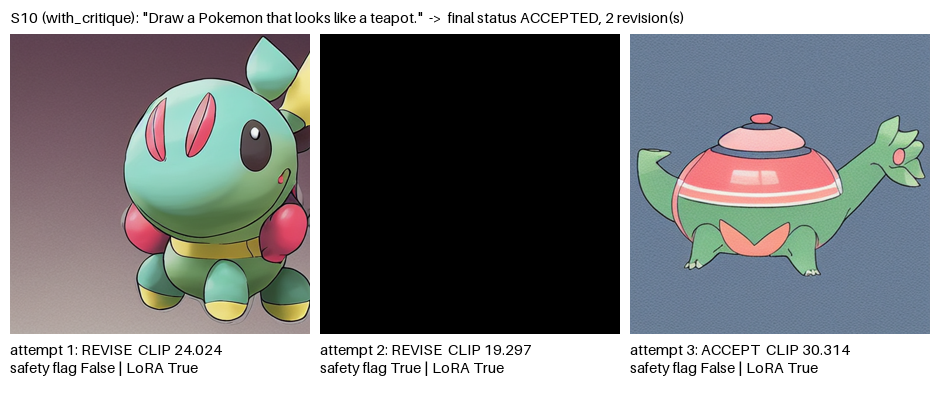
\includegraphics[width=\linewidth]{p3_revision_example_S10.png}
\caption{Recorded revision history of S10 (P3-EXP-003, with critique), built from the saved attempt images and \texttt{result.json}. Attempt~2 was blanked by the safety checker, and the critic revised it rather than accept a blank image.}\label{fig:rev}\end{figure}
Whether critique improves task success can only be decided by the human judgements. \pending{human pass rate with vs.\ without critique; critic--human agreement and Cohen's $\kappa$}

\begin{figure}[t]\centering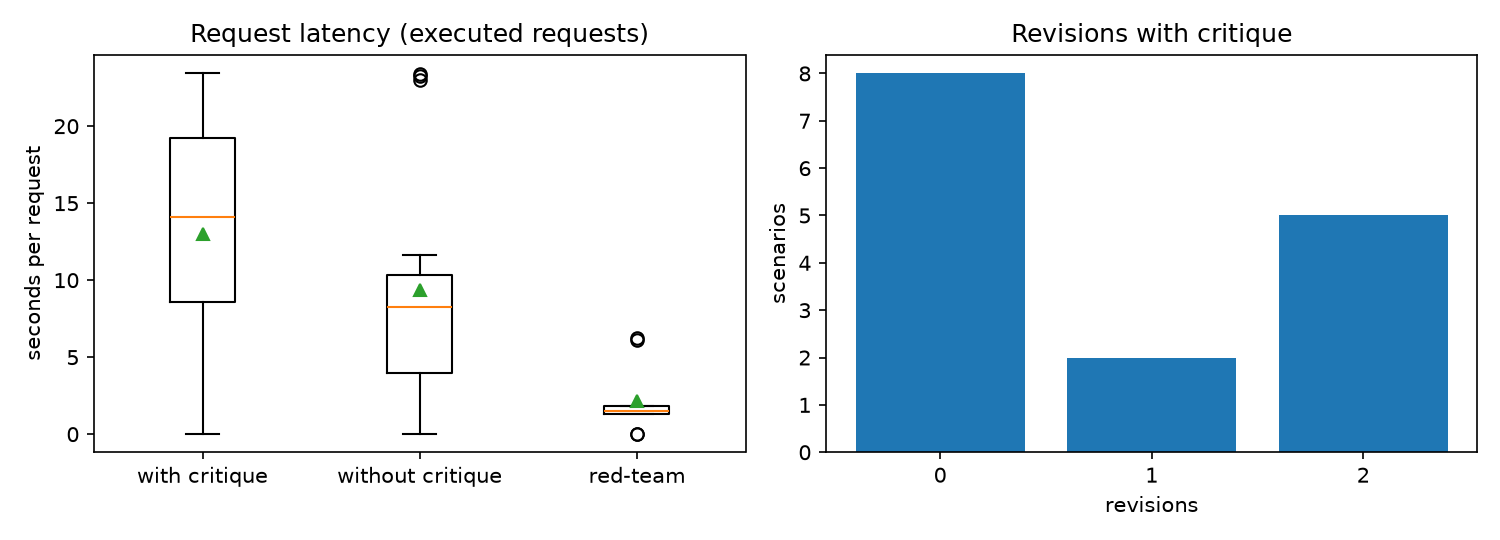
\includegraphics[width=\linewidth]{p3_fig_latency_revisions.png}
\caption{P3-EXP-003 latency per request (left) and revisions per scenario with critique (right).}\label{fig:lat}\end{figure}

\textbf{Red-team.}
\begin{itemize}
\item All 3 unsafe requests and both deceptive real-person edits were refused by the Planner. The broken files ended in FAILED\_INPUT.
\item The image-instruction cases: R03 was refused by the Planner; R01 was refused after injection detection; R02 was answered as a caption while reporting the detected instruction text.
\item R01 and R02 need human review of whether the output follows the hidden text. The confirmed result is 0 attack successes out of the 8 cases decided automatically, with 2 pending. \pending{R01/R02 human verdicts; final attack-success rate out of 10}
\end{itemize}

\textbf{Confirmed failure: Vision-agent repetition loop.}
\begin{itemize}
\item S02, S03 (caption) and S04 (style) failed identically in both conditions.
\item Each vision call generated exactly 1024/1024 tokens without an end-of-sequence token. All 16 successful vision calls stopped at 203--361 tokens (median 235).
\item The locally saved raw replies are valid JSON up to the observed-text list. They then repeat a transcribed sign word, or two alternating words, more than 100 times. This is a deterministic greedy-decoding loop.
\item P3-EXP-002 failed the same way at its 450-token limit, so raising the limit did not help; it only doubled the failure latency to about 23~s.
\item The same loop occurred in the Gradio demo for a newly worded caption request, so it is a general weakness on images with repeated sign text, not a scenario artifact.
\item The pipeline failed closed: no output, a clear error message, and no JSON repair.
\item A fix (repetition control or a deduplicating prompt) was designed but deliberately not run, so the final evidence stays frozen.
\end{itemize}

\subsection{Human evaluation protocol (Part 3)}\label{sec:human3}
Two members judge independently on a blinded packet:
\begin{itemize}
\item 30 scenario folders, both conditions mixed, with the condition hidden; each is marked pass/fail against its rubric.
\item 20 critic attempts, each marked ACCEPT/REVISE, with the critic's decision hidden.
\item The 2 red-team review cases.
\end{itemize}
Disagreements are resolved by discussion and recorded with a rationale. We report percent agreement, Cohen's $\kappa$, pass rates per condition and category, and critic--human agreement. \pending{all human-judged numbers}

\subsection{Gradio demonstration}
The local Gradio app (127.0.0.1:7860 only, \texttt{share=False}) was launched and tested on the final configuration:
\begin{itemize}
\item HTTP 200, and a real request round-trip through Gradio's HTTP API.
\item A watercolor style change ran all five agents and returned an image with a 3-attempt revision gallery (MAX\_REVISIONS, 23.9~s).
\item An unsafe request was refused in 1.4~s.
\item A caption request hit the repetition loop above (FAILED\_MODEL, 25.2~s).
\item The UI shows the status, the selected operation, safety and error messages, per-agent JSON panels, critique feedback, the revision history and the full JSON trace.
\end{itemize}
\pending{UI screenshots: one successful style change, one refusal}

\section{Safety, Ethics and Limitations}\label{sec:limits}
\textbf{Part 1.}
\begin{itemize}
\item \textbf{Unpinned revisions:} the Part~1 model revisions were not pinned.
\item \textbf{Kaggle hardware:} the final notebook ran on a Kaggle T4 within budget (2{,}616~s of 5{,}400~s; at most 4{,}580~MB per model call) with 4-bit NF4 weights, so its answers can differ from the fp16 runs of the earlier checkpoints.
\item \textbf{Memory (historical, P1-EXP-003):} its saved submission run peaked at 18{,}736~MB because the models were loaded twice when the run was repeated in the same kernel. Fresh-kernel runs peaked at 12{,}582~MB (P1-EXP-001, [OUTPUT]) and 12{,}667~MB (P1-EXP-003 run~1, [DOC]).
\item \textbf{No golden-set run of the final notebook:} V14-R1 was not evaluated on the 25-question golden set; the golden-set numbers in Table~\ref{tab:p1} come from earlier code.
\item \textbf{Groundedness not rated:} the planned human groundedness rating was not done. The executed P1-EXP-001 notebook keeps the per-question answers only as truncated tables, and the P1-EXP-003 run-1 answers were not saved; producing them again would need a new run.
\item \textbf{Intermediate versions:} work between P1-EXP-003 and the final notebook (P1-EXP-004 and earlier Kaggle versions) is not preserved as separate commits; only the final V14-R1 notebook and its submission are committed.
\end{itemize}
\textbf{Parts 2--3.}
\begin{itemize}
\item \textbf{Licences:} the training data is CC BY-NC-SA 4.0 and depicts copyrighted characters; SD~1.5 is under CreativeML OpenRAIL-M. Adapters and generated images are for non-commercial research only and must carry the same terms.
\item \textbf{Guardrails:} they rely on English keyword patterns and the VLM's judgements, so paraphrased or obfuscated attacks may pass. Injection detection depends on the VLM reading the image text.
\item \textbf{Safety checker:} it produced false positives (P3-EXP-001's S01, and probably several Part~2 cartoons).
\item \textbf{Repetition loop:} the Vision agent fails on images with repeated sign text (above).
\item \textbf{Metric reliability:} KID uses 20 samples; CLIP is related to SD's text encoder; $\tau{=}25$ is untuned.
\item \textbf{Part~2 human study:} 25 pairs and 3 raters (by design two of them authors) give low power. The selected LoRA~A was preferred in only 38.7\% / 41.3\% of judgments, so the KID-based improvement is not confirmed by humans (Section~\ref{sec:human2}).
\item \textbf{Red-team set:} it was amended after the preliminary run and is not a hold-out.
\item \textbf{16~GB compatibility:} peak allocations were 6.3--6.5~GB (Part~2 training) and 12.5~GB (Part~3) under a 16~GB allocator cap on an RTX 5090. This was \emph{not} tested on real 16~GB hardware (T4/P100, no bf16 on T4).
\end{itemize}

\textbf{Model card summary (Part 2, LoRA A).}
\begin{itemize}
\item SD~1.5 (\texttt{451f4fe1}) with a rank-4 LoRA on the attention projections, 797{,}184 trainable parameters, 1{,}500 steps, 4.0~minutes on an RTX 5090, peak 6{,}307~MB.
\item Adapter sha256 \texttt{20d8d671\ldots}; diffusers format; loaded with \texttt{load\_lora\_weights}.
\item Intended use: non-commercial research in the training style.
\item Limitations: 20-sample KID, outputs pulled toward the training style, and possible resemblance to copyrighted characters.
\item Card files: \texttt{hf\_staging/P2-EXP-001/\{run\_A,run\_B,images\}/README.md} (to be published as \texttt{Parthp01/data266-lab2-lora-a}, \texttt{-lora-b}, \texttt{-generated-images}; \pending{after authorization}).
\end{itemize}

\textbf{System card summary.} Components: Qwen3-VL-4B-Instruct for the planner, vision, prompt, critic and input-safety roles; SD~1.5 with LoRA~A (sha256 \texttt{20d8d671\ldots}), InstructPix2Pix and CLIP ViT-L/14. Intended use: course demonstration of guarded image editing and generation on non-sensitive images. Out of scope: real-person deceptive edits (refused), NSFW content (refused or blocked), and following instructions inside images (never).

\section{Conclusion}
A rank-4 LoRA gave the lowest in-domain KID, at a moderate cost in prompt fidelity and diversity. A rank-64 adapter cost more on both. In a blinded three-rater comparison, however, the rank-4 adapter was preferred over the base model in only 38.7\% (style) and 41.3\% (prompt) of judgments, so the automated improvement was not confirmed by human preference. The five-agent system executed every evaluation request with traceable, bounded behaviour and no confirmed red-team success. One deterministic vision failure mode remains open. Human judgements will determine task success and whether critique helps. \pending{final Part~3 conclusions after the human judgements}

\section*{Contributions and AI Use}
\pending{per-member contributions (see CONTRIBUTIONS.md)}. An AI coding assistant (Claude Code) was used for implementation, documentation and, with team authorization, for executing P3-EXP-003. Details are in \texttt{AI\_USAGE.md}.

\appendices
\section{Evidence sources}
Part~1:
\begin{itemize}
\item the final executed notebook \texttt{notebooks/p1\_rag.ipynb} (P1-KAGGLE-V14-R1; run report in its saved output) and its submission \texttt{eval/p1\_submission.csv};
\item the historical executed notebooks at \texttt{0adebfa} (P1-EXP-001) and \texttt{eb87662} (P1-EXP-003);
\item \texttt{docs/part1/P1\_EXP003\_CHECKPOINT\_MANIFEST.md} and \texttt{docs/part1/DECISIONS\_P1.md};
\item Kaggle scores as recorded by the team [KAGGLE].
\end{itemize}
Part~2: \texttt{\$LAB2\_WORK\_DIR/p2/results/P2-EXP-001/\{report\_summary.json, metrics\_c8d369176621.json, safety\_analysis.json\}}, the run metadata in \texttt{runs/P2-EXP-001/}, and the executed \texttt{notebooks/p2\_finetune.ipynb} (\texttt{FULL\_RUN}). Human evaluation: \texttt{eval/p2\_human\_ratings.csv} (commit \texttt{e53130b}, sha256 \texttt{bc46f0ba\ldots}), scored by \texttt{notebooks/p2\_finetune\_REPORT\_ONLY\_human\_eval.ipynb} (\texttt{report\_summary.json} field \texttt{human}). Post-hoc statistics: \texttt{\$LAB2\_WORK\_DIR/p2/audit/report\_only\_human\_20261118T030113Z/human\_eval\_supplementary\_POSTHOC.json} (D-118).
Part~3: \texttt{\$LAB2\_WORK\_DIR/p3/experiments/P3-EXP-00\{1,2,3\}/evaluation\_summary.json}, per-item \texttt{result.json}, \texttt{traces/P3-EXP-00\{2,3\}/}, the executed \texttt{notebooks/p3\_agents.ipynb}, \texttt{eval/p3\_eval\_freeze\_v2\_P3-EXP-003.json}, and \texttt{DECISIONS.md} (D-105--D-115).

\section{Figure sources}
\begin{table}[h]\centering\footnotesize
\begin{tabular}{ll}\toprule
Figure & Source file (\texttt{\$WORK} = \texttt{data266\_lab2\_work})\\\midrule
\ref{fig:p1arch}, \ref{fig:arch} & drawn in this document (TikZ)\\
\ref{fig:loss} & \texttt{\$WORK/p2/results/P2-EXP-001/figures/loss\_curves.png}\\
\ref{fig:grid} & \texttt{\ldots/figures/grid\_P01.png}, \texttt{grid\_P16.png}\\
\ref{fig:mem} & \texttt{\ldots/figures/memorization\_top3\_runA.png}\\
\ref{fig:lat} & \texttt{\$WORK/p3/experiments/P3-EXP-003/report/fig\_latency\_revisions.png}\\
\ref{fig:rev} & built from \texttt{\ldots/P3-EXP-003/scenario/with\_critique/S10/}\\\bottomrule
\end{tabular}\end{table}
Copies are in \texttt{report/figures/}. Further report-ready figures there: \texttt{p2\_grid\_P11.png}, \texttt{p2\_failure\_candidates\_runA.png}, \texttt{p3\_fig\_automated\_checks\_by\_category.png}.

\begin{thebibliography}{9}
% Team: verify each reference against the original paper before submission.
\bibitem{lora} E.~J.~Hu \emph{et al.}, ``LoRA: Low-rank adaptation of large language models,'' in \emph{Proc. ICLR}, 2022.
\bibitem{ldm} R.~Rombach \emph{et al.}, ``High-resolution image synthesis with latent diffusion models,'' in \emph{Proc. CVPR}, 2022.
\bibitem{kid} M.~Bi\'nkowski \emph{et al.}, ``Demystifying MMD GANs,'' in \emph{Proc. ICLR}, 2018.
\bibitem{clip} A.~Radford \emph{et al.}, ``Learning transferable visual models from natural language supervision,'' in \emph{Proc. ICML}, 2021.
\bibitem{lpips} R.~Zhang \emph{et al.}, ``The unreasonable effectiveness of deep features as a perceptual metric,'' in \emph{Proc. CVPR}, 2018.
\bibitem{ip2p} T.~Brooks, A.~Holynski, and A.~A.~Efros, ``InstructPix2Pix: Learning to follow image editing instructions,'' in \emph{Proc. CVPR}, 2023.
\bibitem{qwen} Qwen Team, ``Qwen3-VL-4B-Instruct,'' model card, \url{https://huggingface.co/Qwen/Qwen3-VL-4B-Instruct}. \pending{cite the official technical report if required}
\bibitem{bge} BAAI, ``bge-large-en-v1.5'' and ``bge-reranker-v2-m3,'' model cards, \url{https://huggingface.co/BAAI}. \pending{cite the official BGE / M3 papers if required}
\bibitem{bm25} S.~Robertson and H.~Zaragoza, ``The probabilistic relevance framework: BM25 and beyond,'' \emph{Found. Trends Inf. Retr.}, 2009.
\bibitem{rrf} G.~V.~Cormack, C.~L.~A.~Clarke, and S.~Buettcher, ``Reciprocal rank fusion outperforms Condorcet and individual rank learning methods,'' in \emph{Proc. SIGIR}, 2009.
\bibitem{data} ``reach-vb/pokemon-blip-captions,'' Hugging Face dataset (CC BY-NC-SA 4.0), revision \texttt{3790f299}.
\end{thebibliography}
\end{document}
